\begin{center}
  \textsf{Листок 4.}
\end{center}
\vspace{0.01cm}
\nopagebreak[2]

\task{ Найти период малых колебаний математического маятника с длиной
  подвеса $l$. Ускорение свободного падения равно $g$.  }

\taskpic{ Длинный железнодорожный состав, двигаясь по инерции,
  въезжает на горку с углом наклом $\alpha$. Когда состав
  полностью остановился, на горке находилась половина его
  длины. Сколько времени прошло от начала подъема до остановки? Длина
  состава $L$, трением пренебречь.}{
  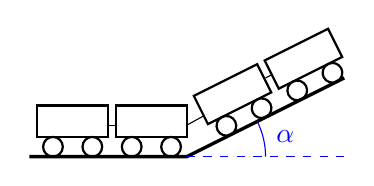
\begin{tikzpicture} 
    \draw[very thick] (0,0) -- (2,0) -- (4,1);
    \draw[blue,dashed] (2,0) -- (4,0);
    \draw[blue] (3,0) arc (0:atan(0.5):1);
    \draw[blue] (3.25,0.25) node {$\alpha$};
    \begin{scope}[thick,xshift=-0.2cm]
      \draw (0.5,0.25/2) circle (0.25/2);
      \draw (1,0.25/2) circle (0.25/2);
      \draw (0.3,0.25) rectangle ++(0.9,0.4);
    \end{scope}
    \draw (1,0.4) -- (1.1,0.4);
    \begin{scope}[thick,xshift=0.8cm]
      \draw (0.5,0.25/2) circle (0.25/2);
      \draw (1,0.25/2) circle (0.25/2);
      \draw (0.3,0.25) rectangle ++(0.9,0.4);
    \end{scope}
    \draw (2,0.4) -- (2.22,0.52);
    \begin{scope}[thick,xshift=1.9cm,yshift=0.95cm,rotate around={atan(0.5):(2,0)}]
      \draw (0.5,0.25/2) circle (0.25/2);
      \draw (1,0.25/2) circle (0.25/2);
      \draw (0.3,0.25) rectangle ++(0.9,0.4);
    \end{scope}
    \draw (3,1) -- (3.08,1.04);
    \begin{scope}[thick,xshift=2.8cm,yshift=1.4cm,rotate around={atan(0.5):(2,0)}]
      \draw (0.5,0.25/2) circle (0.25/2);
      \draw (1,0.25/2) circle (0.25/2);
      \draw (0.3,0.25) rectangle ++(0.9,0.4);
    \end{scope}
\end{tikzpicture}  
}

\task{ На очень шероховатый цилиндр радиуса $r$, расположенный
  горизонтально, надет тонкий однородный обруч радиуса $R$. Найти
  период малых колебаний обруча в вертикальной плоскости.}

\task{ Четыре невесомых стержня длины $L$ каждый соединены шарнирно и
образуют ромб $ABCD$. Шарнир $A$ закреплен, а к шарниру $C$ подвешен
груз. Шарниры $D$ и $B$ соединены невесомой пружиной, имеющей в
недеформационном состоянии длину $1.5L$. В положении равновесия
стержни образуют с вертикалью углы $\alpha=30^{\circ}$. Найти период
малых колебаний $T$ системы.}

\taskpic{ Система, изображенная на рисунке, состоит из стержней,
соединенный шарнирно в точках $A$, $B$, $D$, $E$, $G$ и $F$. В точке
$C$ находится бусинка массой $m$. Точки $B$ и $G$, $F$ и $D$
соединены пружинами жесткостью $k$. В положении равновесия все углы
в системе прямые. Найти период малых колебаний системы.}{
\begin{tikzpicture} 
  \draw[interface,thick] (0,0.5) -- (0,3.5);
  \draw[interface,thick] (3.5,3.5) -- (3.5,0.5);
  \draw[very thick] (0,2) node[right] {$A$} -- (3.5/4,3) node[above]
  {$B$} -- (3.5/2,2) node[above=2] {$C$} -- (3*3.5/4,3) node[above]
  {$F$}  --  (3.5,2) node[left] {$E$};
  \draw[very thick] (0,2) -- (3.5/4,1) node [below] {$G$} -- (3.5/2,2)
  node[below=2] {$m$} -- (3*3.5/4,1) node [below] {$D$}--
  (3.5,2);
  \draw[fill=black] (1.75,2) circle (0.1);
  \begin{scope}
    \draw[very thick] (3.5/4,3) -- (3.5/4,2.5);
    \draw[very thick] (3.5/4,1) -- (3.5/4,1.5);
    \draw[very thick,spring] (3.5/4,2.5) -- (3.5/4,1.5);
  \end{scope}
  \begin{scope}[xshift=3.5/2*1cm]
    \draw[very thick] (3.5/4,3) -- (3.5/4,2.5);
    \draw[very thick] (3.5/4,1) -- (3.5/4,1.5);
    \draw[very thick,spring] (3.5/4,2.5) -- (3.5/4,1.5);
  \end{scope}
  \draw[fill=black] (0,2) circle (0.03);
  \draw[fill=black] (3.5,2) circle (0.03);
\end{tikzpicture}  
}

%%% Local Variables: 
%%% mode: latex
%%% TeX-master: "../../../report"
%%% End: 
